\section{Itération 2: ( 3/8/2017 - 3/28/2017 )}

\subsection{L'objectif du sprint}

La méthodologie Scrum a eu un impact positif sur les développeurs, du point de vue social, elle
a valorisé le travail en équipe, la solidarité, le respect et la communication entre toutes les
parties prenantes (client, développeurs,\ldots). Elle a aussi changé leur vison sur le développement
des logiciels.

L'objectif de cette itération est d'ajouter un système de gestion des rapport, d'améliorer
la qualité de service web de location et d'enrichir des fonctionnalités du ``Dashboard''.
\subsection{Planification de l'itération 2}
  Au sein de la réunion de planification nous avons sélectionné les tâches à réaliser au
  cours de cette itération tout en accord avec le ”Product-Owner”.
  \subsubsection{Backlog de l'itération}
 \begin{center}

    \footnotesize
    \begin{longtable}{| p{1cm} | p{5cm} | p{7cm} | p{1cm} |}
        \caption{backlog de l'itération 2}
        \label{tab:sprint2-backlog} \\

 \hline
 \multicolumn{1}{|c}{\textbf{Réf}} &
 \multicolumn{1}{|c}{\textbf{Spécification}} &
 \multicolumn{1}{|c}{\textbf{Description}} &
 \multicolumn{1}{|c|}{\textbf{Priorité}} \\ \hline
 \endhead

 \hline \multicolumn{4}{|r|}{{Continué en page suivante$\dotsc$}} \\ \hline
 \endfoot

 \hline \hline
 \endlastfoot

\hline
1 & Recherche trajectoire & Notion de trajectoirec & 1 \\ \hline
2 & Affichage du trajet sur la carte&Trajectoire affichée sur la carte d'un ID  & 1 \\ \hline
3 &Réception des données des ralentisseur &Table qui contient les informations des ralentisseur & 1 \\ \hline
4&Responsive design& IHM adaptable & 2 \\ \hline
5 & Ajout un bouton ralentisseur &Enable,Disabled respecte l'IHM  & 2 \\ \hline
6 & Filtrage des marqueurs dans la carte & légende simplifier & 1 \\ \hline
7 & chargement de l'image & Image temporaire dans le serveur jusqu'à la validation & 1 \\ \hline
8 & Enregistrement des informations du rapport dans la BD rapport& Enregistrer les données lors de la validation ou suppression après time-out & 1 \\ \hline
9 & Recherche test unitaires & Comment simplifier le travail en utilisant le test unitaire cote serveur  & 1 \\ \hline
10 & Recherche framework PHP & & 2 \\ \hline 
11 &Groupement des secousse sur la carte & Regrouper les secousses lors d'un zoom out sur la carte & 3 \\ \hline
\end{longtable}
\end{center}

\subsubsection{Estimation de la deuxième itération}
  Comme l'iteration précédant, Nous avons fixé la période de cette itération à 3 semaine
  \begin{table}[htbp]
    \centering
    \begin{tabular}{| c | c | c | c |}
\hline
\textbf{Membre} & \textbf{Nombre d'heures par jour} & \textbf{Nombre de jours présent} & \textbf{Total en heures} \\ \hline
\hline

Moez & 8 & 18& 144\\ \hline
Rihab & 8 & 18 & 144 \\ \hline
\multicolumn{2}{c|}{} & \textbf{Total} & 288 \\ \cline{3-4}
    \end{tabular}
    \caption{Nombre d'heures de travail estimé de l'itération 2}
    \label{tab:sprint2-capacity}
\end{table}
\begin{center}
    \begin{longtable}{| l | l | l |}
        \caption{Nombre d'heures estimé pour la réalisation des taches}
        \label{tab:sprint2-estimation} \\

 \hline
 \multicolumn{1}{|c}{\textbf{Spécification}} &
 \multicolumn{1}{|c}{\textbf{Membre}} &
 \multicolumn{1}{|c|}{\textbf{Heures}} \\ \hline
 \endhead

 \hline \multicolumn{3}{|r|}{{Continué en page suivante$\dotsc$}} \\ \hline
 \endfoot

 \hline \hline
 \endlastfoot

\hline
Recherche trajectoire & Rihab & 5 x 2 \\ \hline
Affichage du trajet sur la carte& Moez & 13 x 2 \\ \hline
Réception des données des ralentisseur& Moez & 5 \\ \hline
Responsive design & Rihab & 5 x 2 \\ \hline
Ajout un bouton ralentisseur& Rihab & 13 x 2 \\ \hline
 Filtrage des marqueurs dans la carte  & Rihab & 13 \\ \hline
chargement de l'image & Moez & 5 \\ \hline
Enregistrement des informations du rapport dans la BD rapport & Moez & 5 \\ \hline
 Recherche test unitaires & Moez & 5 \\ \hline
Recherche framework PHP & Moez & 5 \\ \hline
Groupement des secousse sur la carte  & Rihab & 5 \\ \hline
\end{longtable}
\end{center}
\subsubsection{Évaluation du travail}
\subsection{Présentation des outils utilisés}

\subsubsection{Lumen}

Pour le développement de backend du notre plateforme, la langue du programmation
PHP a été pré choisi. Mais, on avait la responsabilité de choisir les
bibliothèques et les frameworks. Pendant la 1\iere{} itération, le but était de
se familiariser avec la langue PHP. Donc, on a utilisé seulement les extensions
officiel du PHP incluant PDO, $\dotsc$ . Dans l'itération suivante, on a étudié
les frameworks disponibles. A la fin, on a choisi le framework Lumen qui est
une version simplifié du Laravel pour le développement des API \acrshort{RESTful}.
\TODO{ARAVEL , sYNFONY,slim COMPARAISON }


\subsection{Mises des normes}

Les critaires à respecter pour cette itération sont:

\paragraph{Qualité d trajectoire}
Le trajectoire doit être aligné sur le trajet avec bonne précision. Et le nombre
des positions nécessaire pour tracer le trajectoire doivent être le minimum le
plus possible.

\paragraph{Architecture modulaire}
Architecture de back-end doit étre modulaire: On doit changer notre code
procédurale par un code orienté objet et minimiser la duplication du code et
séparer le code des models et le code des controlleurs.

\paragraph{IHM de la page Dashboard Responsive}
Affiche claire et responsive des marqueurs dans la carte meme si le nombre est
trés élevé.

\subsection{Modélisation UML}

\begin{figure}[htbp]
  \centering
  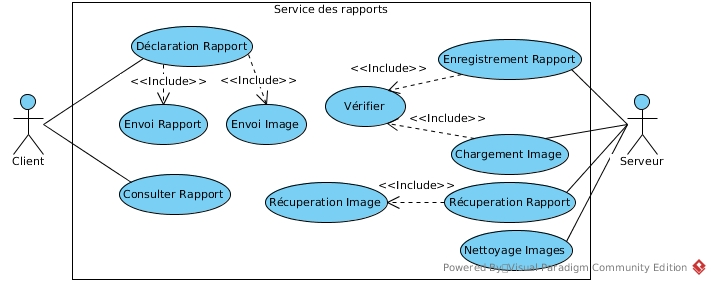
\includegraphics[width=1\textwidth]{sprint2-webservices-report-usecase}
  \caption{Diagramme de case d'utilisation du services Rapports en itération 2}
\end{figure}

\begin{figure}[htbp]
    \centering
    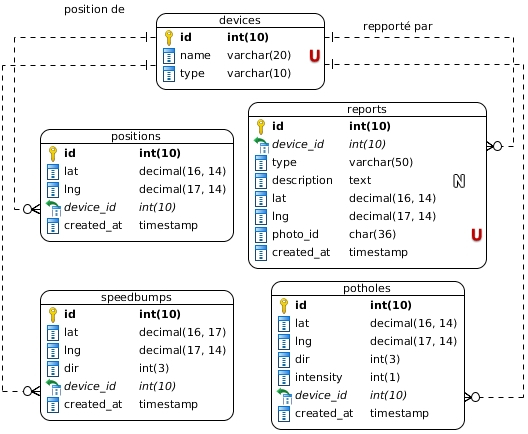
\includegraphics[width=1\textwidth]{sprint2-webservices-database}
    \caption{Diagramme entité-association du service Position en itération 2}
\end{figure}

\begin{figure}[htbp]
  \centering
  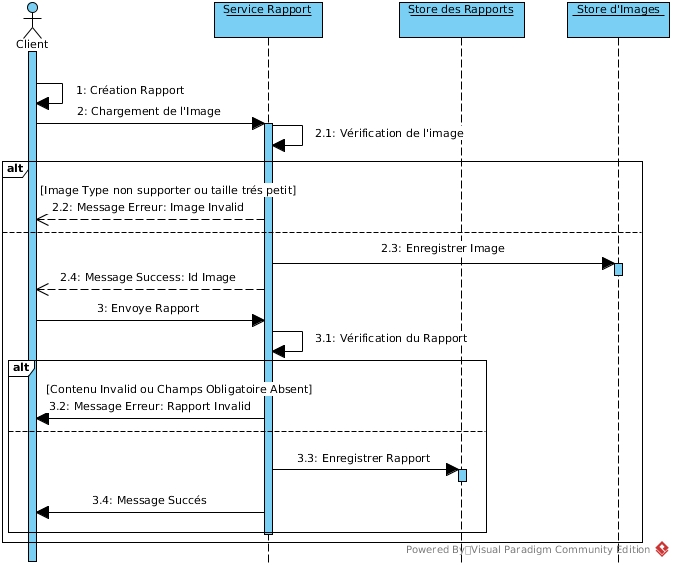
\includegraphics[width=1\textwidth]{sprint2-webservices-report-post-sequence}
  \caption{Diagramme de séquence du services Post Rapports en itération 2}
\end{figure}

\begin{figure}[htbp]
  \centering
  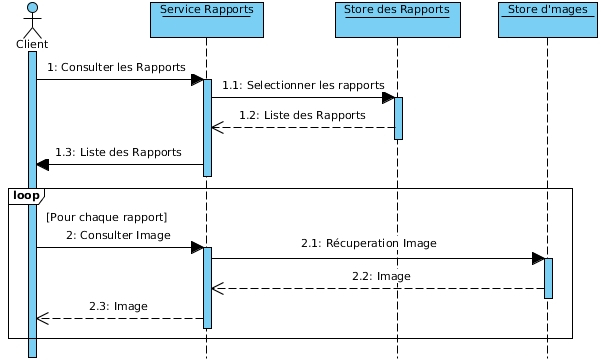
\includegraphics[width=1\textwidth]{sprint2-webservices-report-get-sequence}
  \caption{Diagramme de séquence du services Get Rapports en itération 2}
\end{figure}

\subsection{Évaluation suivant les normes mise}

\TODO{EVALUATION}

\subsection{Contributions}

\TODO{Rewrite Front end js}

\subsection{Revue de cette itération}
\subsubsection{Produit de l'itération}

A la fin de l'itération 2,nous détaillons les différentes spécifications qui
caractérisent et implémenté le systeme de gestion des rapport.

\paragraph{Page \textquote{Rapport}}

Dans cette page, nous donne la main à l'utilisateur pour faire un petit rapport
comme expliqué dans la figure~\ref{fig:sprint2-rapport-screenshot1}.
Cette page permet à l'utilisateur d'envoyer son rapport au serveur pour
l'enregistrer.
La position du rapport est détecté automatique à travers l'api JavaScript
standard Location. On donne la main à l'utilisateur pour changer la location
manuellement en glissant le marqueur ou en changer les inputs.
Le chargement de l'image est obligatoire.
\TODO{Cette obligation était éliminer en review}

L'envoie du rapport est éxecuté en deux phases:
\begin{enumerate}
    \item Chargement de l'image au serveur. Si le type et le taille de l'image
        est valide, le serveur retourne un id unique (UUID) de l'image.
    \item Envoie du rapport au serveur. Les informations envoyées sont: type du rapport, id image, commentaire (optionnel) et les coordonnées.
\end{enumerate}

\begin{figure}[htbp]
  \centering
  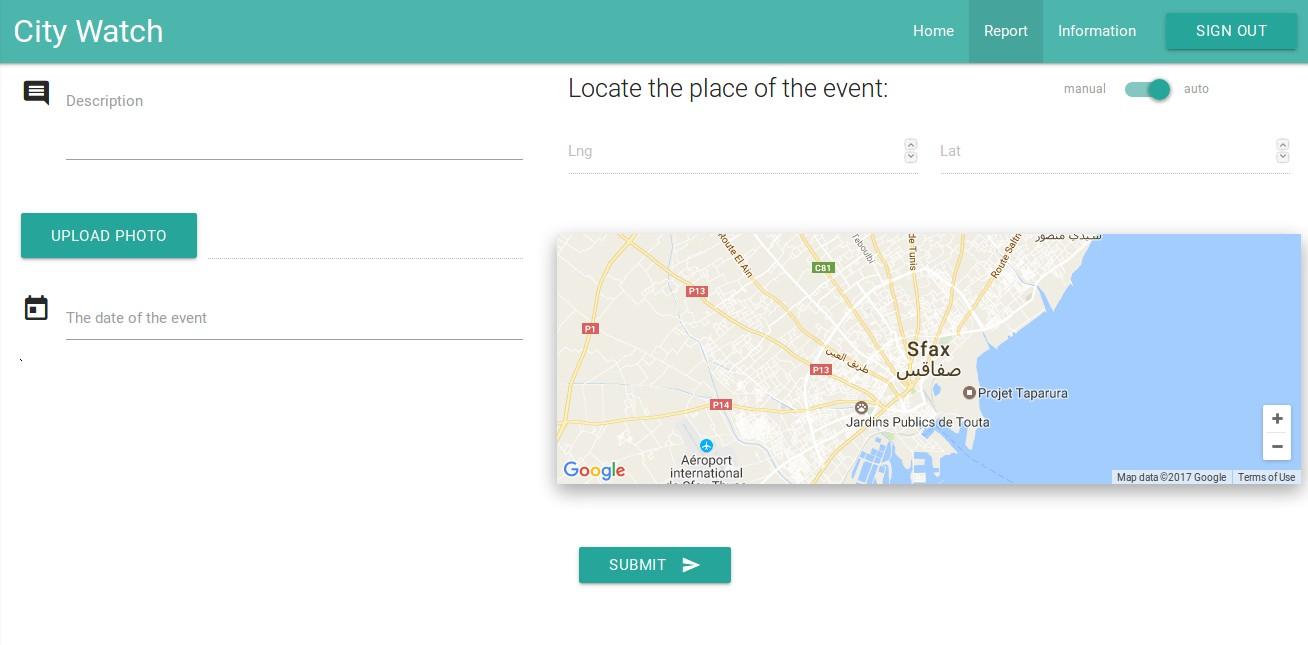
\includegraphics[width=0.7\textwidth]{sprint2-rapport-screenshot1}
  \caption{Page Rapport}
  \label{fig:sprint2-rapport-screenshot1}
\end{figure}
\paragraph{Page \textquote{Dashboard}}
L'utilitaire de regroupement de marqueurs vous aide à gérer plusieurs marqueurs à différents niveaux de zoom.
Précisément, les  marqueurs  sont en fait des éléments à ce stade et ne deviennent réellement des
marqueurs qu'après leur rendu. Par souci de clarté, nous ne parlerons que de marqueurs 
dans ce document.

Lorsqu'un utilisateur affiche la carte à un niveau de zoom élevé comme montre la
figure~\ref{fig:sprint2-dashboard-screenshot1}, les différents marqueurs
s'affichent sur la carte. Lorsqu'il effectue un zoom arrière comme montre la
figure~\ref{fig:sprint2-dashboard-screenshot2}, les marqueurs se regroupent pour faciliter la consultation de la carte.

\begin{figure}[htbp]
    \begin{subfigure}{.5\textwidth}
    \centering
  \centering
  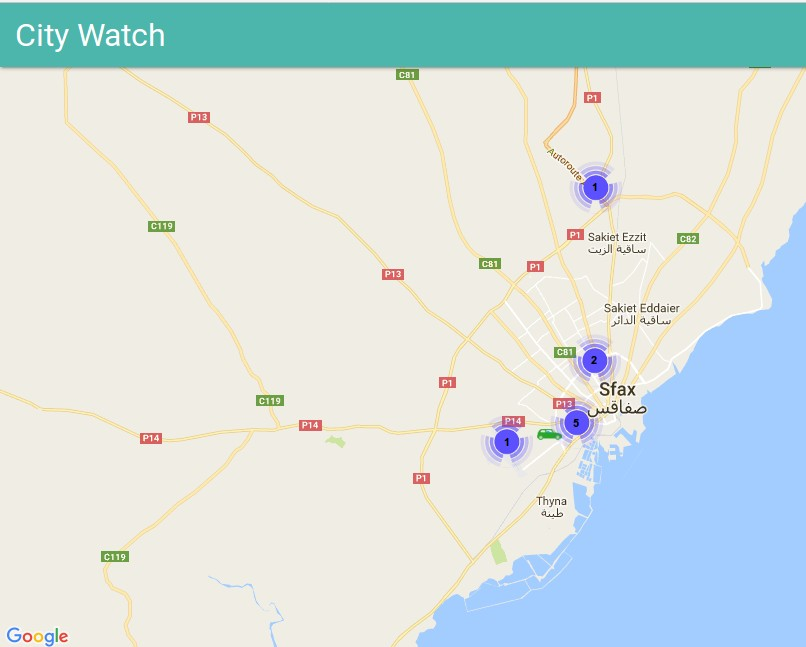
\includegraphics[width=.8\linewidth]{sprint2-dashboard-screenshot1}
  \caption{Groupement activé en un zoom bas}
  \label{fig:sprint2-dashboard-screenshot1}
\end{subfigure}
\begin{subfigure}{.5\textwidth}
    \centering
  \centering
  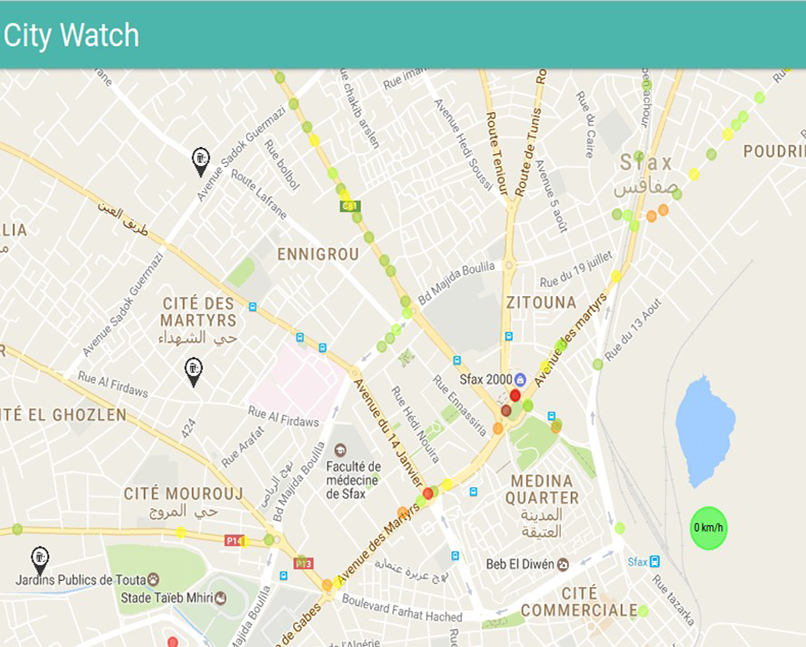
\includegraphics[width=.93\linewidth]{sprint2-dashboard-screenshot2}
  \caption{Groupement désactivé en zoom haut}
  \label{fig:sprint2-dashboard-screenshot2}
\end{subfigure}
\caption{Groupement des marqueurs des secousses en diffenet niveaux du zoom}
\end{figure}

\paragraph{"Application Mobile ``CityWatch''}
\TODO{ Description}
\begin{figure}[htbp]
    \begin{subfigure}{.5\textwidth}
    \centering
  \centering
  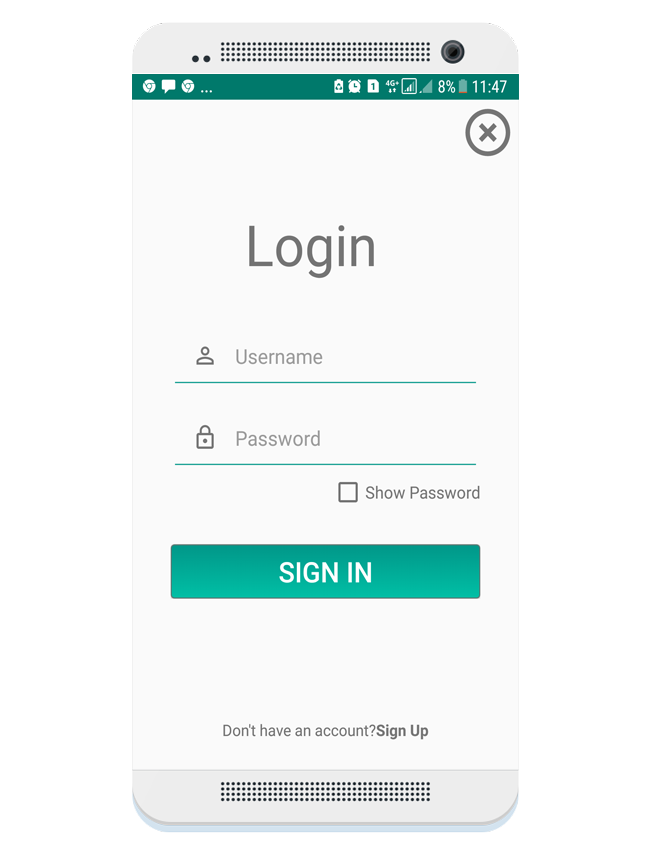
\includegraphics[width=.8\linewidth]{sprint2-android-screenshot1}
  \caption{Activity login}
  \label{fig:sprint2-android-screenshot1}
\end{subfigure}
\begin{subfigure}{.5\textwidth}
    \centering
  \centering
  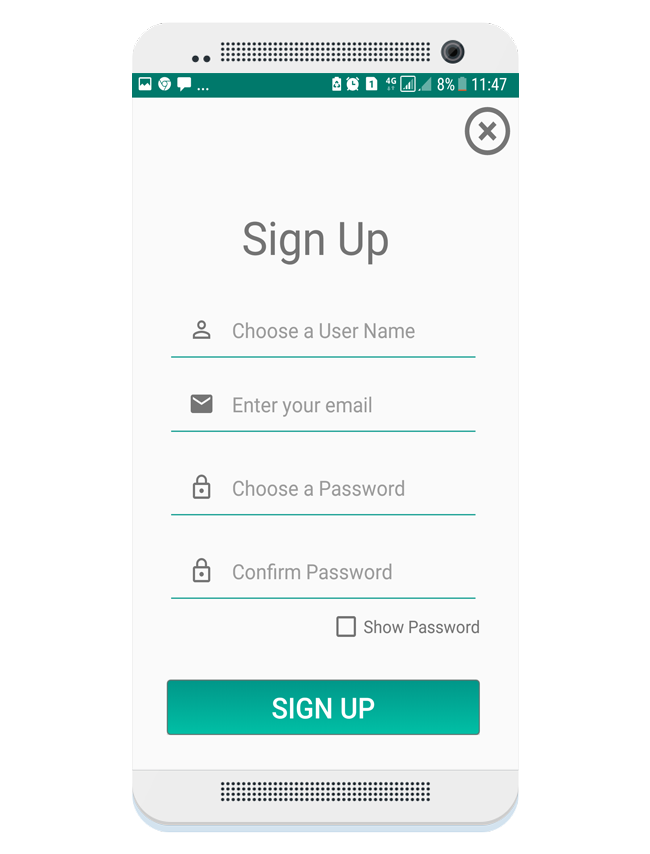
\includegraphics[width=.8\linewidth]{sprint2-android-screenshot2}
  \caption{Activity sing up}
  \label{fig:sprint2-android-screenshot2}
\end{subfigure}
\caption{xxxxxxxxxxxxxxxxxxxxxxxxxxxxxxx}
\end{figure}

\subsubsection{Avis du ProductOwner}
A la fin de cette première itération, nous avons présenté au ”Product Owner” le produit
obtenu. Le ”Product-Owner” a exprimé sa satisfaction du travail.

\subsubsection{Burndown de l’itération}
\usetikzlibrary{plotmarks}

\begin{figure}
\centering
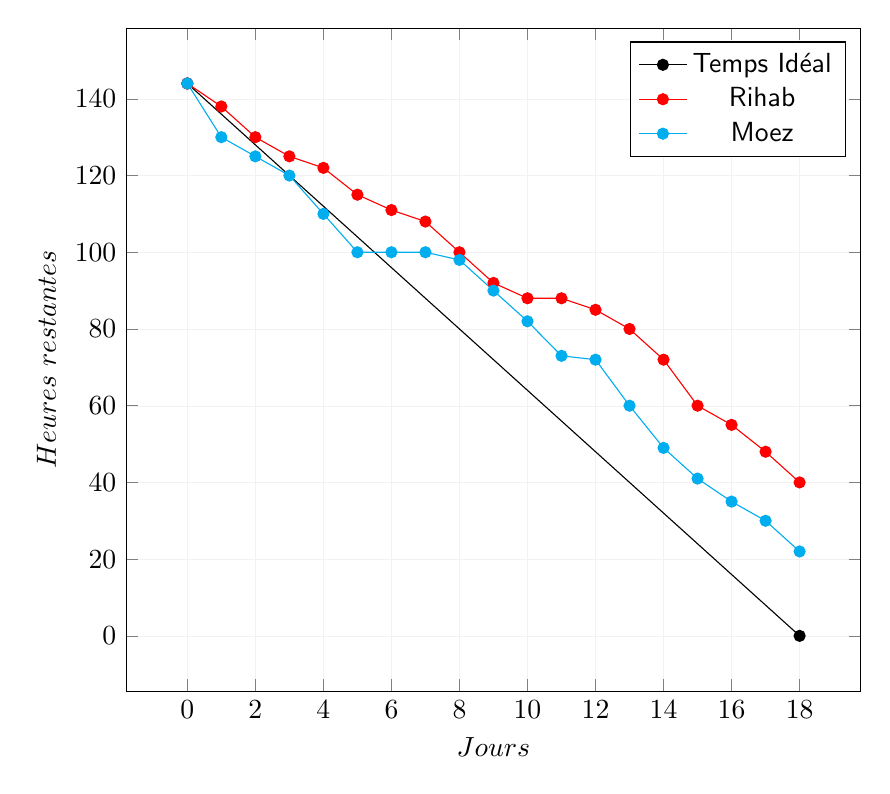
\begin{tikzpicture}[y=.1cm, x=.7cm,font=\sffamily]
\begin{axis}[
xlabel=$Jours$,
ylabel=$Heures\ restantes$,
grid=both,
grid style={line width=.1pt, draw=gray!10},
width=0.9\textwidth,
height=10cm,
%major grid style={line width=.2pt,draw=gray!50},
]
\addplot[color=black,mark=*] coordinates {
        (0,144)
        (18,0)
    };
    \addlegendentry{Temps Idéal}

    \addplot[mark=*,red] plot coordinates {
        (0, 144)
        (1, 138)
        (2, 130)
        (3, 125)
        (4, 122)
        (5, 115)
        (6, 111)
        (7, 108)
        (8, 100)
        (9, 92)
        (10, 88)
        (11, 88)
        (12, 85)
        (13, 80)
        (14, 72)
        (15, 60)
        (16, 55)
        (17, 48)
        (18, 40)
       
    };
    \addlegendentry{Rihab}
      \addplot[mark=*,cyan] plot coordinates {
        (0, 144)
        (1, 130)
        (2, 125)
        (3, 120)
        (4, 110)
        (5, 100)
        (6, 100)
        (7, 100)
        (8, 98)
        (9, 90)
        (10, 82)
        (11, 73)
        (12, 72)
        (13, 60)
        (14, 49)
        (15, 41)
        (16, 35)
        (17, 30)
        (18, 22)
       
    };
    \addlegendentry{Moez}
\end{axis}
\end{tikzpicture}
\caption{Graphique d'avancement - Itération 2}
\end{figure}
